%avoid page number on blank pages when cleared
\thispagestyle{empty}
\cleardoublepage  
\chapter{METODOLOG\'IA DE LA SOLUCI\'ON}
\label{chap:methodology}

En este cap\'itulo se presenta la metodolog\'ia general de la soluci\'on,
que consiste en las diferentes etapas de procesamiento de im\'agenes que deben ser
llevadas a cabo para detectar eficazmente la forma de gusanos C. elegans presentes
en im\'agenes digitales. Primero, se presenta una descripci\'on general de la 
metodolog\'ia, donde se justifica el dise\~no de la soluci\'on y se presentan los 
diferentes procesos involucrados.
Luego, se explica cada proceso de manera individual, aclarando su respectiva utilidad y necesidad.
Por cada proceso se presenta, adem\'as, las caracter\'isticas de su implementaci\'on en este trabajo,
lo que da origen al algoritmo que aqui se provee.

\section{Dise\~no de la Metodolog\'ia: Razonamiento Previo}
\label{sec:reasoning}

Como se explica en \cite{binaryshape,deformable,matching2,matchingbook},
uno de los enfoques mas comunes para el ajuste de formas consiste en adoptar
un descriptor de forma, construir una silueta a partir del descriptor,
y posicionar dicha silueta lo suficientemente cerca del objeto a ajustar en
la imagen. Seguidamente, variar los valores de los par\'ametros 
del descriptor, deformando la silueta inicial, hasta que se logre una 
coincidencia aceptable entre la silueta generada y el objeto en la imagen.\\
 
La utilizaci\'on de un descriptor de forma suele ser apropiado
cuando los objetos a ser ajustados pueden ser categorizados
en un clase espec\'ifica, y pueden ser descritos
en t\'erminos geom\'etricos.
El problema de estudio tiene como objetivo la detecci\'on y ajuste
de gusanos, particularmente aquellos que pertenece a la especie
C. elegans. Dado la propiedad vermiforme de estos individuos, los
objetos a detectar pueden ser agrupados en una \emph{clase gusano},
a la que pertenecer\'ian aquellos objetos que cumplen con las propiedades
geom\'etricas de tener una forma: alargada, delgada y cil\'indrica, en
t\'erminos generales.
Siguiendo esta idea, se puede definir un descriptor que 
permita generar siluetas de gusanos. Este descriptor podr\'ia
estar representado por dos puntos extremos (los extremos del gusano)
y un conjunto de valores de grosor a lo largo del eje medio que
conecta dichos extremos. Luego, el problema quedar\'ia
reducido a encontrar cada par de puntos extremos de gusanos en la
imagen, ubicar una silueta aproximada (constru\'ida a trav\'es
del descriptor de forma) cerca del gusano a ajustar, y deformar 
la silueta hasta encontrar una coincidencia factible.\\

Para este estudio, las im\'agenes de entrada consisten, b\'asicamente, en
tomas de microscopio de un conjunto de gusanos agrupados en medio 
l\'iquido. Las im\'agenes pueden contener algo de ruido tal como: 
sombras, burbujas de aguas o peque\~nos restos que no pertenecen a
los gusanos, y que por tanto deben ser separados del resto de la imagen. La
posici\'on de cada gusano individual en la imagen es variable y puede
ser distinguida en dos grandes grupos: agrupaciones de gusanos y gusanos aislados.
Una agrupaci\'on de gusanos corresponde a un conjunto de gusanos que aparecen en la
imagen solap\'andose entre si. De esta manera, cada gusano que pertenece
a la agrupaci\'on esta conectado con el resto de manera directa o indirecta,
 a trav\'es de solapamiento. O lo que es lo mismo, desde cada gusano en la agrupaci\'on,
se puede trazar un camino hacia otro gusano sin pasar por p\'ixeles de fondo.  
Por otro lado, los gusanos aislados, son aquellos que estan rodeados por
p\'ixeles de fondo y que no se solapan con ning\'un otro gusano.\\

Los diferentes gusanos aislados y agruaciones de gusanos podr\'ian ser
separados f\'acilmente del resto de la imagen, permitiendo as\'i, 
procesar cada uno individualmente. El contorno de los gusanos aislados
puede ser trazado f\'acilmente siguiendo los pixeles del objeto que
estan mas cercanos a los p\'ixeles de fondo. Habiendo ajustado las formas
de gusanos aislados, estas podr\'ian utilizarse para generar un perfil
de gusano, que definir\'ia los valores generales para un descriptor de forma
g\'enerico. Esto permitir\'ia describir la silueta que mejor se ajusta a todos
los gusanos de la imagen, en general.
Los gusanos que pertenecen a agrupaciones de gusanos, se podr\'ian detectar
individualmente, a trav\'es de un proceso de ajuste de siluetas como
el mencionado al comienzo de esta secci\'on.

\section{Descripci\'on de la Metodolog\'ia e Implementaci\'on}
\label{met:description}

\subsection{Descripci\'on General}

La metodolog\'ia presenta un dise\~no general por etapas, 
independiente de la implementaci\'on particular de cada una de estas. De esta
manera, se presenta una visi\'on general de la soluci\'on, y as\'i diferentes
algoritmos pueden ser desarrollados que se ajusten a esta metodolog\'ia.
Se provee, adem\'as, un enfoque espec\'ifico de implementaci\'on por etapa, que da
origen al algoritmo que fue implementado y probado en este trabajo.\\

Siguiendo el razonamiento de la secci\'on anterior, se dise\~n\'o una metodolog\'ia tomando en cuenta
los aspectos principales del proceso de detecci\'on y ajuste de formas estudiado, como lo son:
identificaci\'on general de gusanos en la imagen, segmentaci\'on de gusanos, 
descriptor de forma de gusanos y optimizaci\'on del ajuste de formas.

A continuaci\'on, se describe la metodolog\'ia de la soluci\'on de forma general,  y
seguidamente se explica cada etapa de forma detallada.
En la Figura \ref{fig:methsol} se presenta una descripci\'on gr\'afica de la metodolog\'ia.\\

\begin{figure}[h t b p ! H]
 \centering
   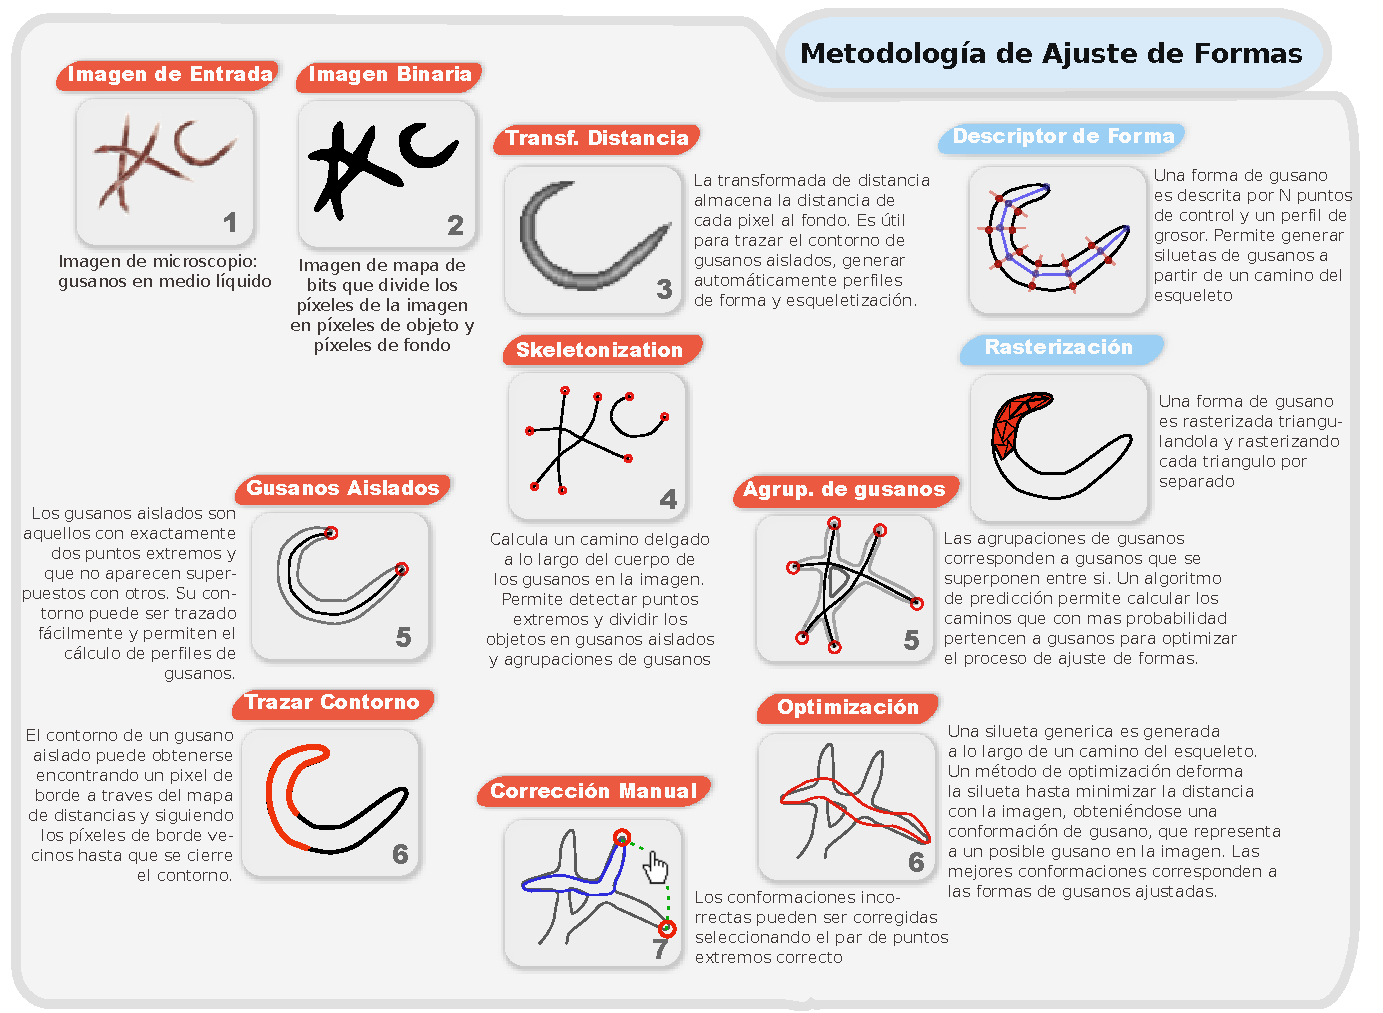
\includegraphics[scale=0.9,angle=270]{diagrams/design.pdf}
 \caption{Descripci\'on gr\'afica de la metodolog\'ia para detectar gusanos C. elegans
   en im\'agenes digitales}
\label{fig:methsol}
\end{figure}

Dada la im\'agen de entrada, el primer paso consiste en separar los p\'ixeles que
pertenecen a los objetos de estudio (gusanos) del resto de la imagen. Para esto,
se utiliza alg\'un m\'etodo del valor umbral (MVU) que permita calcular una imagen
binaria que separe p\'ixeles de gusanos de los p\'ixeles del fondo. Por lo general,
este proceso no es completamente eficaz, y se obtiene algo de ruido en la imagen, el
cual debe ser eliminado en procesamientos posteriores. Esta primera etapa corresponde
a una segmentaci\'on inicial de la imagen de entrada.
Seguidamente, a partir de la imagen binaria, se puede calcular una transformada de
distancia o mapa de distancias, en la cual se almacena la distancia de cada p\'ixel
al p\'ixel de fondo mas cercano. La transformada de distancia hace posible identificar
f\'acilmente los p\'ixeles de contorno en la imagen binaria, lo que la convierte en
una herramienta fundamental para la generaci\'on autom\'atica de perfiles de gusanos,
el trazado de contornos en gusanos aislados y para la optimizaci\'on del proceso
de \emph{esqueletizaci\'on}, entre otros. \\

Habiendo determinado los p\'ixeles que pertenecen a gusanos en la imagen, se pueden separar
los grupos de p\'ixeles que estan conectados y rodeados por p\'ixeles de contorno. Esta
segmentaci\'on provee diversos grupos de p\'ixeles objetos. Cada uno de estos grupos
podr\'ia ser tanto un gusano aislado como una agrupaci\'on de gusanos, de acuerdo a la diferenciaci\'on
expuesta en la Sec. \ref{sec:reasoning}.
Una manera de diferenciar los diferentes grupos es contando el n\'umero de extremos y de intersecciones. 
Un grupo que contiene extactamente dos puntos extremos y que
no presenta intersecciones corresponder\'a a un gusano aislado. Por otro lado, si el grupo presenta
mas de dos puntos extremos, o al menos una intersecci\'on, esto indicar\'a la presencia de 
solapamiento de gusanos, por tanto correspondar\'a a una agrupaci\'on de gusanos.\\

El enfoque de ajuste de formas se centra en ubicar incialmente una silueta de gusano gen\'erica 
cerca de un posible gusano en la imagen. De esta manera, es necesario poder determinar, con cierto grado
de precisi\'on y factibilidad, \'areas que pertenezcan a gusanos individuales en la imagen. Para este prop\'osito,
el esqueleto topol\'ogico de la imagen, proveer\'ia un camino continuo a trav\'es del eje medio
de los objetos inicialmente segmentados, conectando puntos extremos de gusanos. Al mismo tiempo, permitir\'ia
detectar gran cantidad de puntos extremos.\\

Seguidamente, los diferentes grupos segmentados son procesados para detectar 
y ajustar la forma de los gusanos individuales que los conforman.
Los dos tipos de grupos definidos (agrupaciones de gusanos y gusanos aislados),
son procesados de formas diferentes. 

\subsubsection*{Gusanos Aislados}
El contorno de la silueta de los gusanos aislados puede ser trazada f\'acilmente de 
la siguiente forma: se selecciona un pixel de contorno (indicado en el mapa de distancias)
y se construye un camino siguiendo el pixel de contorno vecino en cada paso, hasta que
se cierre el contorno. Luego, la silueta puede ser \emph{rasterizada} construyendo 
una maya triangulada y, seguidamente, rasterizando cada triangulo por separado. Esto
proveer\'ia el conjunto de los p\'ixeles que pertenecen a la forma del gusano, por lo que
la forma quedar\'ia ajustada.\\
El ajuste casi perfecto que se puede obtener de los gusanos aislados, hace posible
calcular un perfil de gusano que represente a los individuos de la muestra, de forma
general. De esta manera, se puede construir un descriptor de forma preciso (esto 
es explicado a fondo en la secci\'on \ref{sec:metshapedescriptor}).

\subsubsection*{Agrupaciones de Gusanos}
Para detectar los gusanos individuales presentes en una agrupaci\'on de gusanos, 
se calculan las formas de gusanos factibles entre par de puntos extremos y luego 
se determina cuales de aquellas tienen m\'as probabilidades de pertenecer a gusanos 
en la imagen. \\

El proceso en general es como sigue: dado un par de puntos extremos, se selecciona
alg\'un camino entre ellos. Luego, se escogen un conjunto de puntos control y
apartir de estos puntos y del descriptor de forma, 
se genera una silueta de gusano alrededor del camino. Dicho camino constituye el 
eje medio de la silueta generada. Despu\'es de esto, se lleva a cabo un proceso de 
ajuste de formas, que consiste en minimizar la distancia que existe entre la silueta
generada y el gusano que presumiblemente se encuentra dispuesto en un espacio 
cercano al camino escogido, hasta que el mejor ajuste es encontrado. Una forma ajustada,
despues del proceso de minimizaci\'on, se denomina conformaci\'on. Una conformaci\'on 
corresponde a la mejor silueta de gusano que se puede construir a partir de un camino
entre dos extremos determinados, y que presumiblemente representa a un gusano real
de la imagen. \\

Este proceso es repetido para cada camino de gusanos factible que puede ser encontrado
a partir de cada punto extremo. De esta manera, se obtienen todas las conformaciones
posibles en el imagen. Luego, un algoritmo de asignaci\'on permitir\'a seleccionar
el mejor conjunto de conformaciones, que maximice el n\'umero de puntos extremos cubiertos
y minimice el valor acumulado de energ\'ia. Las conformaciones escogidas incorrectamente
a trav\'es de la asignaci\'on automaticamente, podran ser corregidas siguiendo
un sencillo proceso manual.\\

Un algoritmo de predicci\'on de caminos puede ser utilizado para encontrar
los caminos de gusano mas probables, que parten de un punto extremo dado.
Las conformaciones resultantes de los caminos predichos por el algoritmo podr\'ian
ser beneficiados sobre otras conformaciones, para aumentar la probabilidad de que
sean escogidos.\\

En las secciones siguientes se cubren detalladamente los diferentes procesos
involucrados en la metodolog\'ia presentada, y se presenta el enfoque particular
de implementaci\'on seguido en este trabajo, para cada uno de ellos.
  

\subsection{Segmentaci\'on Inicial (M\'etodo del Valor Umbral)}
\label{sec:metthres}

Dado que el prop\'osito principal de este estudio es detectar y ajustar la forma de 
gusanos C. elegans en im\'agenes digitales, un paso inicial fundamental es el de separar
las formas de gusanos lo mas posible del resto de la im\'agen, para asi poder llevar a
cabo un anal\'isis mas preciso.\\

Sean los gusanos en la imagen los objetos a separar y considerando el resto de la imagen
como fondo o segundo plano, los p\'ixeles de la imagen puede ser separados en dos grupos: 
p\'ixeles de objeto y p\'ixeles de fondo. Dada esta caracterizaci\'on, un m\'etodo del valor
umbral permitir\'ia separar los objetos en la imagen digital y descartar la informaci\'on
innecesaria, representando esto a trav\'es de una imagen binaria. La imagen binaria proveer\'ia
entonces una segmentaci\'on inicial de la imagen original, siendo ademas clave para el
calculo del mapa de distancias de la imagen, como se explica en la Sec. \ref{sec:metdt}.
En general, para esta etapa de la metodolog\'ia, cualquier MVU que permita obtener una imagen
binaria que identifique satisfactoriamente los p\'ixeles que pertenecen a los gusanos de la
imagen, ser\'a suficiente para continuar el proceso normalmente, sin importar la existencia
de ruido leve en la im\'agen.


\subsubsection*{Implementaci\'on}
\label{sec:thresimp}

Existen cuatro MVU para im\'agenes en 2D implementados en \emph{Endrov},
estos son: \emph{Fukunaga}, \emph{entrop\'ia m\'axima}, \emph{Otsu} y \emph{percentil},
que cubren las categor\'ias de MVU basados en histogramas y MVU basados en entrop\'ia 
(ver Sec. \ref{sec:thresholding}). Dada la condici\'on de transparencia de los gusanos
C. elegans, es dificil determinar teoricamente cual vendr\'ia a ser el m\'etodo mas apropiado 
para obtener una imagen binaria precisa. \\
Por esta raz\'on, se realizaron una serie de experimentos
para seleccionar el m\'etodo mas apropiado. Estos experimentos consistieron en el ajuste manual
de los diferentes par\'ametros de cada uno de los m\'etodos mencionados, que fueron aplicados
sobre un conjunto de imagenes de prueba. La precisi\'on de segmentaci\'on de las im\'agenes binarias
obtenidas en cada caso, se midi\'o a trav\'es de una comparaci\'on visual con la imagen original.\\
El m\'etodo que mejor se comport\'o en estos experimentos resulto ser el 
\emph{m\'etodo del valor umbral por percentil}, 
al ser el mas f\'acil de ajustar manualmente y aquel que retorn\'o el equivalente binario mas preciso, 
en cada caso. Un an\'alisis mas detallado sobre la escogencia del m\'etodo de valor umbral para esta metodolog\'ia
se presenta en la secci\'on de experimentos del cap\'itulo cuatro (ver Sec. \ref{chap:experiments}).\\

En la figura \ref{fig:wormthres} se presenta una imagen binaria, obtenida al
aplicar el \emph{m\'etodo del valor umbral por percentil}.

\begin{figure}[h t b p ! H]
  \centering
  \subfloat[Imagen original]{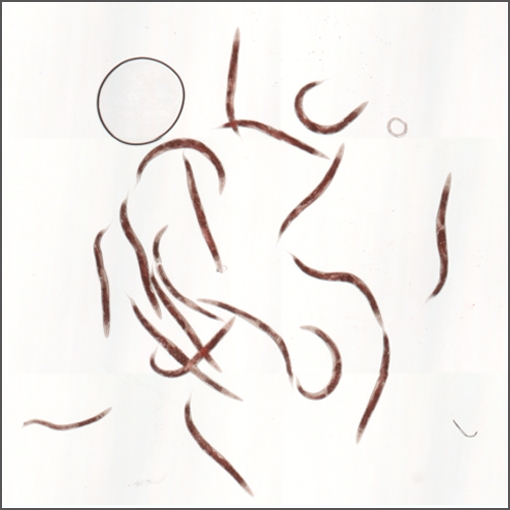
\includegraphics[width=0.45\textwidth]{original.png}}
\qquad
  \subfloat[M\'etodo del valor umbral por percentil. Valor=0.074]{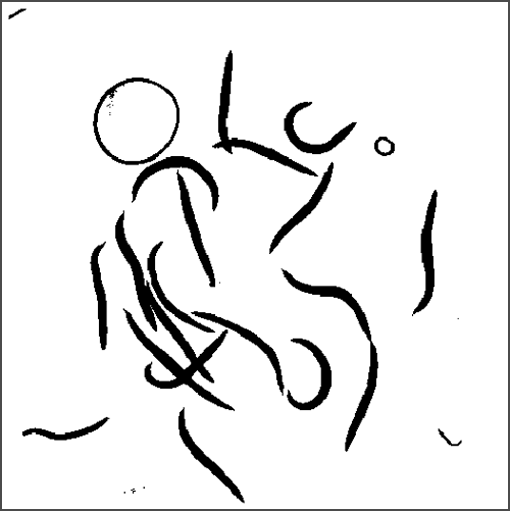
\includegraphics[width=0.45\textwidth]{thres/worms}}
\caption{Gusanos en medio l\'quido. Imagen original e imagen binaria obtenida a trav\'es
del m\'etodo del valor umbral por percentil, con un percentil de 0.074}
  \label{fig:wormthres}
\end{figure}

\subsection{Transformada de Distancia}
\label{sec:metdt}

La transformada de distancia de la imagen binaria es utilizada a fondo en el
seguimiento de contorno y en diferentes tipos de procedimientos de segmentaci\'on.
Espec\'ificamente, el mapa de distancias permite detectar y delinear el contorno
exacto de gusanos aislados (Sec. \ref{sec:metiso}), es \'util en la generaci\'on
automatica de perfiles de gusanos (Sec. \ref{sec:metwormprof}), y es esencial en 
la predicci\'on heur\'istica de caminos de gusanos mas probables (Sec. \ref{sec:pathguessing}). 
As\'i mismo, permite mejorar el rendimiento de algoritmo iterativo de reducci\'on de capas
dise\~nado por \emph{Zhang y Suen}, \cite{thinning}, como se describe en 
la Sec. \ref{sec:metsk}

\subsubsection*{Implementaci\'on}
\label{sec:dtimp}

Tal como se describe en \cite[p.196]{fastdt}, los algoritmos para calcular transformadas de distancia pueden ser
categorizados en dos grandes clases: m\'etodos iterativos y metodos secuenciales o recursivos. 
Los m\'etodos iterativos son particularmente eficientes en computadoras de arreglos celulares
dado que se pueden procesar todos los p\'ixeles en paralelo en cada iteraci\'on. Por otro lado, los m\'etodos secuenciales
se ajustan mejor a computadoras convencionales, al evitar iteraciones por ser independientes del tama\~no de los objetos.
Tomando en cuenta los tipos de computadoras a la que tienen acceso la mayor\'ia de las personas que trabajan
en el procesamiento de im\'agenes digitales, los algoritmos secuenciales ofrecen un rendimiento mucho mas
eficiente que los iterativos. Por esta raz\'on, se escogi\'o un enfoque secuencial para calcular la 
transformada de distancia de las im\'agenes de entrada. Particularmente se utiliz\'o el algoritmo de
transformaci\'on de dos recorridos con vecindarios de 3x3, presentado en \cite{fastdt}, que es
tanto eficiente como sencillo de implementar.\\

En el trabajo antes mencionado, se describe un algoritmo para calcular el mapa 
de distancias de una imagen en formato de mapa de bits, que consite en dos recorridos y
una operaci\'on por p\'ixel. La complejidad del algoritmo es $\mathcal{O}(N)$, donde $N$ 
es el tama\~no del arreglo que contiene la imagen.
En dicho trabajo se presenta, inicialmente, un pseudo-c\'odigo para las m\'etricas 
de distancia de \emph{Manhattan} y \emph{tablero de ajedrez}, \cite[p.197]{fastdt}.
Luego, la definici\'on es extendidad para mejorar la eficiencia de los c\'alculos 
requeridos para generar un mapa de distancias a trav\'es de la metrica de distancias
\emph{Euclideanas}, \cite[p.198]{fastdt}.
Este algoritmo de dos recorridos, fue implementado utilizando las tres m\'etricas de
distancia mencionadas anteriormente. Esto permite realizar una an\'alisis mas amplio
del comportamiento y precisi\'on del proceso de ajuste de formas, al cambiar de
una metrica a la otra. Esto es debido a que los mapas de distancia generados por 
diferentes m\'etricas, representan a los objetos de maneras diferentes, y tienden
a ser sensible a cambios posicionales u otras propiedades. En \cite[p.332]{eucskeleton}
se asegura que las m\'etricas de \emph{tablero de ajedrez} y \emph{Manhattan} son
sensibles a las rotaciones de los objetos, mientras que la m\'etrica \emph{Euclideana}
permanece invariable ante estas rotaciones; sin embargo, es mucho mas costosa de calcular.\\

Dada la forma alargada y estrecha de los gusanos C. elegans, y los diferentes niveles
de precisi\'on que proveen dichas m\'etricas de distancia, es dif\'icil decidir
cual se ajusta mejor al problema de estudio, por lo que debe ser determinado
experimentalmente. La Figura \ref{fig:distance} muestra una im\'agen binaria y tres
mapas de distancia obtenidos a partir de una imagen que contiene, \'unicamente, un
gusano aislado.

\begin{figure}[h t b p ! H]
  \centering
  \subfloat[Imagen Binaria]{\label{fig:manh}
\includegraphics[width=0.35\textwidth]{dt/binary}}
\qquad
  \subfloat[Distancia de Manhattan]{\label{fig:manh}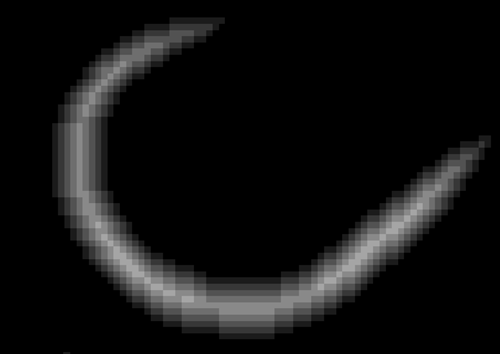
\includegraphics[width=0.35\textwidth]{dt/manhattandt}}
\qquad                
  \subfloat[Distancia de tablero de ajedrez]{\label{fig:chess}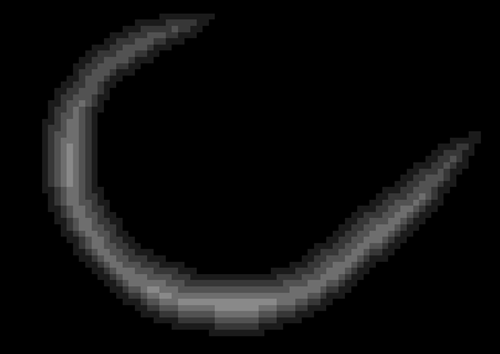
\includegraphics[width=0.35\textwidth]{dt/chessboarddt}}
\qquad
  \subfloat[Distancia Euclideana]{\label{fig:mouse}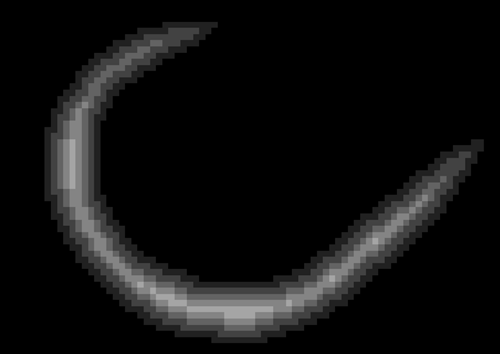
\includegraphics[width=0.35\textwidth]{dt/euclideandt}}
  \caption{ Imagen binaria y tres mapas de distancia utilizando diferentes m\'etricas,
    a partir de la imagen de un gusano}
  \label{fig:distance}
\end{figure}

\subsection{\emph{Esqueletizaci\'on}}
\label{sec:metsk}

La \emph{esqueletizaci\'on} de la imagen corresponde al proceso de obtener un 
camino de p\'ixeles conectado y delgado, que tienda
al eje central o eje medio de los gusanos en la imagen. A este camino se le
denomina esqueleto. Este es un proceso
clave en el enfoque de detecci\'on presentado en este trabajo, tal como
se enuncia incialmente en la Sec \ref{met:description}. El esqueleto de la
imagen hace posible identificar la cantidad de gusanos presentes, permite
diferenciar y separar las agrupaciones de gusanos de los gusanos aislados, 
y mas importante, provee caminos entre extremos de gusanos (que tienden
al eje medio). Estos caminos son fundamentales en el proceso de ajuste
de formas (ver Sec \ref{sec:metsegmentation}), pues proveen informaci\'on
acerca de la localizaci\'on de los gusanos en la imagen, al constituir trayectorias
a lo largo de las cuales podr\'ian estar dispuestos gusanos en la imagen.

\subsubsection*{Implementaci\'on}
\label{sec:skeletonimp}


Para los efectos de este trabajo, el algoritmo de \emph{esqueletizaci\'on} a ser
seleccionado debe garantizar la conectividad de los puntos del esqueleto, \emph{i.e.}
cada punto del esqueleto debe estar conectado con al menos otro punto del mismo
esqueleto. As\'i mismo, el esqueleto debe ser tan delgado como sea posible 
(hasta un 1 p\'ixel de grosor) para simplificar el procesamiento y an\'alisis de caminos.\\

Existen diferentes m\'etodos que consisten en encontrar los puntos cresta en el
mapa de distancias y conectarlos, como se explica en \cite{maxima,euclideancentre,ridgedt}. 
El enfoque presentado en \cite{maxima} fue seguido inicialmente para calcular un esqueleto
de imagen delgado en un tiempo de ejecuci\'on muy corto. Pese a que el estudio garantiza
que el algoritmo permite calcular, satisfactoriamente, esqueletos conectados de un pixel
de grosor, este result\'o ser eficaz \'unicamente para los gusanos aislados. Los esqueletos
obtenidos para agrupaciones de gusanos resultaron generalmente desconectados, 
de mas de un p\'ixel de grosor y poco precisos. Estos llevo a la utilizaci\'on
de un enfoque diferente.\\

En \cite{thinning} se presenta un algoritmo iterativo para calcular el esqueleto de
una imagen binaria. El algoritmo consiste, b\'asicamente, en la remoci\'on por capas
de aquellos pixeles que, de acuerdo a determinados criterios, no pertenecen al esqueleto
del objeto. El dise\~no del algoritmo esta dirigido a computadoras con procesadores 
paralelos, de manera que se puedan ejecutar varias operaciones de pixel al mismo tiempo,
y mejorar as\'i el rendimiento. Para evitar el requerimiento de utilizar computadores
con procesadores paralelos, sin desmejorar el rendimiento significativamente,
el algoritmo fue ligeramente modificado. Dicha modificaci\'on consiste en utilizar
el mapa de distancias para descartar chequeo de p\'ixeles que pertenecen a capas
mas profundas que la capa que esta siendo reducida en un momento determinado.
Esto toma ventaja de la naturaleza de los mapas de distancia, quienes, por definici\'on,
establecen capas de distancia entre los p\'ixeles del objeto y el fondo de la imagen.\\
De esta manera, las capas se definen por el valor que tiene cada p\'ixel en el mapa 
de distancias. La primera capa corresponde a un valor de distancia de uno ($1$), la segunda
un valor de dos ($2$) y as\'i sucesivamente. El algoritmo es presentado en \ref{thinninalg}.

\begin{algorithm}                     
\caption{Calculate shape skeleton}         
\label{thinninalg}                    
\begin{algorithmic}                   
\STATE $shapePts \leftarrow getBinaryObjectPixels()$
\STATE $dtImage \leftarrow getImageDistanceMap()$
\STATE $contourIndex \leftarrow 1$
\STATE $makeThinner = True$

\WHILE{$makeThinner$}

\STATE \COMMENT{remove south-east boundary points and the north-west 
corner point}
\FOR{$pixel$ in $shapePts$}
\IF{$dtImage(pixel) > contourIndex$}
\STATE \COMMENT{skip iteration}
\ELSE
\STATE $pixelRemove \leftarrow southEastCondition(pixel)$
\IF{$pixelRemove$}
\STATE $shapePts.remove(pixel)$
\STATE $makeThinner \leftarrow True$
\ENDIF

\ENDIF
\ENDFOR

\STATE \COMMENT{remove the north-west boundary points and the
		south-east corner points}
\FOR{$pixel$ in $shapePts$}
\IF{$dtImage(pixel) > contourIndex$}
\STATE \COMMENT{skip iteration}
\ELSE
\STATE $pixelRemove \leftarrow northWestCondition(pixel)$
\IF{$pixelRemove$}
\STATE $shapePts.remove(pixel)$
\STATE $makeThinner \leftarrow True$
\ENDIF
\ENDIF
\ENDFOR
\ENDWHILE
\STATE 
\RETURN{$shapePts$}

\end{algorithmic}
\end{algorithm}

El algoritmo se ocupa bien de los gusanos que se solapan, al construir un camino que 
se aproxima bien al eje central de las figura, y resulta en un esqueleto totalmente
conectado y delgado (mayoritariamente 1-pixel de grosor).
En la Figura \ref{fig:skeleton} se presenta el esqueleto de un conjunto de gusanos.

\begin{figure}[h t b p ! H]
 \centering
   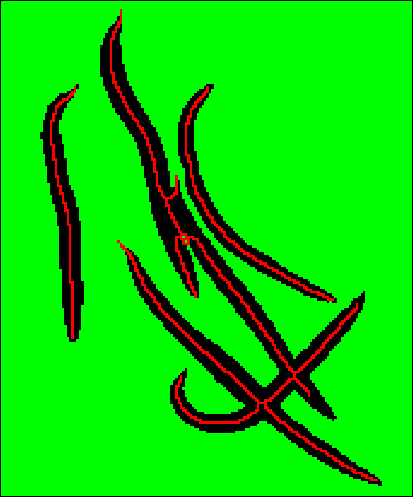
\includegraphics[scale=0.75]{skeleton/skeleton.png}
 \caption{Esqueleto obtenido a trav\'es de reducci\'on por capas iterativa
   de un conjunto de gusanos}
\label{fig:skeleton}
\end{figure} 

\subsection{Segmentaci\'on de Gusanos}
\label{sec:metsegmentation}

Dado que el objetivo es ajustar las formas de gusanos individuales, es 
necesario localizarlos en la imagen y separarlos lo m\'as posible, 
\emph{i.e. }segmentar la imagen. La segmentaci\'on de los objetos 
de estudio permite mejorar la eficiencia y precisi\'on del proceso
de ajuste de formas, al reducir el area a analizar, disminiyuendo as\'i
la cantidad de combinaciones diferentes que deben ser tomadas en cuenta.
Una vez que se han identificado los puntos extremos, se pueden calcular
los diferentes caminos que existen entre ellos a partir del esqueleto.
A trav\'es del conjunto de puntos extremos y de la cantidad de caminos e 
interesecciones, se puede determinar el tipo de grupo de gusanos al que
pertenece cada grupo de objetos segmentados, ya sean gusanos aislados
o agrupaciones de gusanos. De esta manera, el proceso de ajuste de formas
se puede llevar a cabo en cada grupo por separado.\\

Otro proceso de segmentaci\'on que debe ser llevado a cabo es la identificaci\'on
de caminos de gusanos individuales, tanto para gusanos aislados como para agrupaciones
de gusanos. Estos son caminos que no tiene bifurcaciones y que comienzan y terminan
en puntos extremos.\\
El esqueleto de un gusano aislado determinado corresponde a un camino de este tipo, y es
utilizado para dos procesos diferentes: encontrar el contorno del gusano aislado 
(ver Sec. \ref{sec:metiso}) y generar un perfil de gusanos (ver Sec. \ref{sec:metwormprof}).
El perfil de gusanos permite definir una representaci\'on general de los gusanos en 
la imagen. De esta manera, a trav\'es del perfil y un camino entre dos extremos, se puede
construir una silueta de gusano, que tiene como eje central al camino escogido. \\

Con respecto a las agrupaciones de gusanos, se deben encontrar caminos de gusanos factibles entre
pares de puntos extremos. Si un camino existe entre un par de puntos extremos, ser\'a posible
generar un conformaci\'on de gusano valida a trav\'es del proceso de optimizaci\'on. 
Estos caminos pueden ser escogidos tanto calculando todas las combinaciones de caminos posibles
entre par de puntos extremos, como a trav\'es de un algoritmo de predicci\'on de caminos probables,
como el que se describe mas adelante en esta secci\'on.

\subsubsection{Implementaci\'on}

\subsubsection*{Puntos Extremos de Gusanos}
\label{sec:wend}

A partir del esqueleto calculado se pueden detectar puntos extremos 
de gusanos. Aquellos p\'ixeles del esqueleto que estan conectados
(son vecinos) de dos o m\'as p\'ixeles se denominan p\'ixeles de cuerpo.
Estos p\'ixeles de cuerpo pertenecen al esqueleto pero no son extremos.
Por otro lado, los puntos extremos del esqueleto son aquellos que estan conectados con
un solo p\'ixel y pueden corresponder al extremo de un gusano, aunque no
necesariamente.\\

Dado que el algoritmo de \emph{esqueletizaci\'on} de reducci\'on por capas
no permite asegurar que los extremos identificados pertenezcan a extremos
de gusanos en la imagen, se debe llevar a cabo un proceso de expansi\'on
del esqueleto, para alcanzar los puntos extremos reales.
El algoritmo se fundamenta en estirar los extremos del esqueleto, siguiendo
una direcci\'on coherente, hasta alcanzar puntos de contorno que vendr\'ian a 
representar los extremos de los gusanos. El algoritmo de expansi\'on utiliza
la definici\'on de \emph{vecino direccional}, que se presenta en \cite[p.334]{maxima}.
Un p\'ixel $D$ es \emph{vecino direccional} de otro p\'ixel $P$, si pertenece a
la vecindad de $P$ (\emph{8-vecindad}) y est\'a localizado dentro de un rango de 
$\pm$ $45^{\circ}$  de cambio de pendiente, con respecto a la orientaci\'on actual
del camino recorrido hasta $P$. En la Figura \ref{fig:directional} se presentan 
tres ejemplos de vecindades direccionales.\\
El algoritmo consiste en seguir el mejor camino direccional, partiendo de cada
punto extremo y expandiendo el esqueleto, hasta que un punto de contorno es
encontrado.
 
\begin{figure}[h t b p ! H]
 \centering
   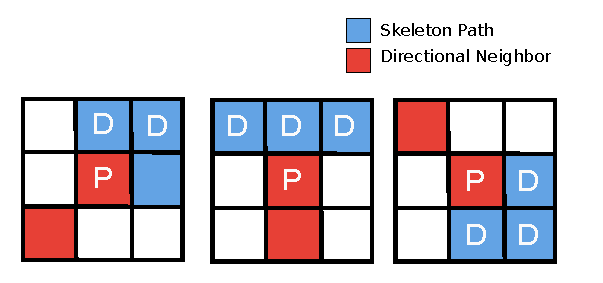
\includegraphics[scale=1]{skeleton/directional.pdf}
 \caption{Tres vecindades direccionales}
 \label{fig:directional}
\end{figure}

El algoritmo de expansi\'on de esqueleto puede ser resumido en 
los siguientes pasos:

\begin{itemize}
\item Seleccionar un punto extremo.
\item Encontrar el p\'ixel de esqueleto anterior y calcular la
  vecindad direccional.
\item Seleccionar el vecino direccional con el menor valor en el
  mapa de distancia y marcarlo como p\'ixel de esqueleto.
\item Si el vecino seleccionado no es un punto de contorno, repetir
  el proceso.
\end{itemize}

Seguidamente se lleva a cabo un proceso de remoci\'on de p\'ixeles de objeto 
incorrectos, que consiste en eliminar aquellos esqueletos cuyo tama\~no (en 
cantidad de p\'ixeles) sea menor que un umbral determinado. Esto permite remover
regiones ligeramente ruidosas, as\'i como punto extremos incorrectos.
Una vez que el esqueleto ha sido expandido satisfactoriamente, los puntos
extremos del esqueleto son marcados como puntos extremos de gusanos.\\

Es importante considerar que, en algunos casos, hay puntos extremos de gusanos
que no puede ser detectados a trav\'es del proceso previamente descrito. 
Particularmente en imagenes con gran cantidad de gusanos, donde existe
una alta posibilidad de que los solapamientos entre gusanos oculten
puntos extremos. Para solucionar esto, se puede llevar a cabo un proceso
manual de adici\'on de puntos extremos faltantes, como se explica en 
la Sec. \ref{sec:manualproc}.


\subsubsection*{Segmentaci\'on en Grupos}


Habiendo detectados los puntos extremos de los diferentes grupos de esqueletos
en la imagen, se puede identificar a que tipo de grupo de gusano corresponde cada uno:
ya sea agrupaciones de gusanos o gusanos aislados. Esto se hace identificando
los extremos de gusanos que estan unidos a trav\'es de un camino del esqueleto.
Como se explic\'o previamente, los gusanos que se superponen son considerados 
parte de un objeto en com\'un en la imagen binaria, por lo que los puntos
extremos que pertenecen a los esqueletos de agrupaciones de gusanos se encuentran
conectados a trav\'es de un camino del esqueleto.\\

Basado en este razonamiento, se dise\~n\'o un algoritmo que detecta la cantidad de
puntos extremos que son conectados a trav\'es de caminos de un determinado esqueleto,
y determina el tipo de grupo de gusanos al que pertenece. Aquellos esqueletos donde
se conectan exactamente dos puntos extremos a trav\'es de uno y solo un camino, corresponde
a gusanos aislados. Mientras que los esqueletos en donde mas de dos puntos extremos son
conectados corresponden a agrupaciones de gusanos.
Este procedimiento es descrito en el Algoritmo \ref{groupsegment}. 

\begin{algorithm}[h]                     
\caption{Calculate shape skeleton}         
\label{groupsegment}                    
\begin{algorithmic}                   

\STATE $endPtList \leftarrow$ list of endpoints
\STATE $clusterIndex \leftarrow$ 0
\FOR{$endpoint$ in $endPtList$}
\IF{$endpoint.wasVisited()$}
\STATE \COMMENT{skip iteration}
\ELSE
\STATE $clusterIndex +=1$
\STATE $followPath(endpoint,clusterIndex)$
\ENDIF
\ENDFOR
\end{algorithmic}
\end{algorithm}

\begin{algorithm}[h]                     
\caption{Follow Path algorithm ( $followPath(currentPoint,clusterCount)$ )}         
\begin{algorithmic}                   

\REQUIRE $currentPoint$
\REQUIRE $clusterCounter$

\IF{not $currentPoint.isSkeletonPoint()$}
\RETURN 
\ELSE
\STATE $addToCluster(endpoint,clusterIndex)$
\ENDIF

\STATE \COMMENT{continue tracing path}
\IF{$currentPoint.isEndPoint()$}
\STATE $markEndPointAsVisited(currentPoint)$
\ENDIF
\STATE $neighbors \leftarrow getNeighborhood()$
\FOR{$n$ in $neighbors$}
\STATE $followPath(endPoint,clusterCounter)$
\ENDFOR

\end{algorithmic}
\end{algorithm}


\subsubsection*{Predicci\'on de Caminos}
\label{sec:pathguessing}

Una agrupaci\'on de gusano es definida por un esqueleto
que conectan puntos extremos a trav\'es de caminos. Sin embargo, hasta esta etapa,
se desconoce el par de puntos extremos que pertenecen a cada gusano en la imagen, y 
el mejor camino en el esqueleto
que conecte a cada par, y que mejor represente el eje central de cada gusano 
respectivo.\\

El algoritmo de optimizaci\'on, cubierto en la Sec. \ref{sec:metfit}, lleva a cabo un
proceso de manipulaci\'on de siluetas para ajustar formas de gusanos en la imagen, dados
dos puntos extremos y un camino que los conecte. Para calcular la forma de gusano mas probable
que parte de un punto extremo determinado, el algoritmo tendr\'ia que probar cada camino posible
que parte de dicho punto extremo y seleccionar el que mejor se ajuste, lo que tiende a traducirse  
en un alto costo en tiempo de ejecuci\'on.\\
Con el fin de reducir el tiempo de ejecuci\'on del algoritmo de ajuste de
formas, y as\'i mismo proveer un par\'ametro adicional para determinar la
factibilidad de los caminos analizados, se desarroll\'o un algoritmo de
predicci\'on de caminos. En s\'intesis, el agoritmo lleva a cabo una b\'usqueda
heur\'istica para determinar aquellos caminos que tienen mayor probabilidad
de representar a un gusano de la imagen.\\

El algoritmo de predicci\'on se basa en la idea de evitar caminos que
tienden a describir conformaciones no-naturales de gusanos. Para esto
es necesario identificar cambios abruptos en el camino y flexiones
poco com\'unes o imposibles en gusanos. La idea desarrollada para lograr
esto se centra en que cada paso siguiente que sea seleccionado, corresponda
a la direcci\'on mas coherente con respecto al camino que ha sido
trazado hasta ese momento. 
Mas espec\'ificamente, se escoge el conjunto $S$ de los \'ultimos $N$ 
pasos trazados, y a partir de este, se calcula la direcci\'on mas com\'unmente
seguida en esa porci\'on del recorrido.\\

Una dificultad considerable que surge de este
enfoque, es que el seguimiento del camino tiende a evitar \emph{centros de bifurcaciones}.
Una bifurcaci\'on ocurre cuando mas de un camino diferente puede ser seguido a partir
de un punto determinado. Dado que estas bifurcaciones son originadas por solapamiento 
de gusanos, el \'area de la bifurcaci\'on suele ser grande, y por tanto hay mayor 
cantidad de p\'ixeles posibles a escoger como siguiente paso. Los \emph{centros de bifurcaciones}
son aquellos puntos que se ubican en la zona mas c\'entrica de estas \'areas, y por tanto
se encuentran a una distancia normalmente similar de todos los caminos que se bifurcan.
Para poder determinar con mayor precisi\'on el camino mas adecuado a seguir, el trazado del camino 
debe tender a los \emph{centros de bifurcaciones}. Sin embargo, siguiendo el enfoque presentado, estos
centros se tienden a bordear. Por esta raz\'on se desarroll\'o una heur\'istica, que permita
al recorrido tender hacia los \emph{centros de bifuraciones} y llevar as\'i a una 
decisi\'on mejor informada.\\

La heur\'istica consiste b\'asicamente en considerar el valor en el mapa de distancias
del p\'ixel elegible, multiplicado por un factor de equilibrio. De esta manera, la 
selecci\'on del p\'ixel siguiente se basa en dos valores fundamentales: la cantidad
de veces que ha sido escogida la direcci\'on en la que se encuentra dicho p\'ixel, 
en los \'ultimos $N$ pasos, y el valor de la heur\'istica para ese p\'ixel. Esto
puede expresarse de la siguiente forma:

$$Siguiente(p) = \max_{s \in vecindad(p)} (valorDir(direccion(p,s),N) + td(n)*factorH)$$

donde $p$ es el \'ultimo p\'ixel marcado, $valorDir$ es una funci\'on que calcula
la cantidad de veces que la direcci\'on del p\'ixel vecino $s$ ha sido escogida, $td$ es el 
mapa de distancia y $factorH$ es el factor heur\'istico que controla la influencia 
del mapa de distancia.\\


El Algoritmo \ref{guess} presenta un pseudo-c\'odigo para este enfoque de predicci\'on
de caminos de gusanos.

\begin{algorithm}[h]                    
\caption{Pseudo-code algorithm for path guessing between endpoints}         
\label{guess}                    
\begin{algorithmic}                   

\STATE $endPtList \leftarrow$ list of endpoints
\STATE $wc \leftarrow$ paths and endpoint in worm cluster 
\STATE $length \leftarrow$ worm estimated length multiplied by a scaling factor
\FOR{$endPoint$ in $endPtList$}
\IF{$alreadyReached(endPoint)$}
\STATE \COMMENT{skip iteration}
\ENDIF
\STATE{$markAsReached(endPoint)$}

\STATE $path \leftarrow$ empty list

\STATE $reachedEndPoint \leftarrow False$
\STATE $currentPixel \leftarrow endPoint$
\WHILE{$not(reachedPoint)$ and $size(path)<length$}
\STATE $currentPixel \leftarrow getBestNeighbor(currentPixel)$
\STATE $updateDirectionsArray(direction(currentPixel))$
\STATE $path.add(currentPixel)$
\IF{$isEndPoint(currentPixel)$}
\STATE $reachedEndPoint \leftarrow True$
\ENDIF
\ENDWHILE 

\IF{$not(reachedEndPoint)$}
\IF{number Of Reachable Endpoints $= 0$}
\STATE $createEndPoint(currentPixel)$
\STATE $path.add(currentPixel)$
\ELSE
\STATE \COMMENT{Select a path to reachable endpoint}
\ENDIF
\ENDIF
\ENDFOR

\end{algorithmic}
\end{algorithm}

\subsection{Descriptor de Forma}
\label{sec:metshapedescriptor}

Como se mencion\'o inicialmente en la Sec. \ref{met:description}, 
el enfoque metodol\'ogico dise\~nado se basa en la manipulaci\'on de 
siluetas de gusanos que se generan a partir de un descriptor de forma.
La forma de un gusano puede ser descrita en t\'erminos geom\'etricos
como objetos alargados, delgados y cil\'indricos. Dado que el proceso
de esqueletizaci\'on y la posterior segmentaci\'on de la imagen, hacen
posible obtener caminos entre pares de extremos de gusanos, un descriptor
de forma permitir\'ia construir siluetas de gusanos a lo largo del
eje central definido por el camino, lo que servir\'ia como par\'ametro
de entrada para el algoritmo de ajuste de formas.\\


El descriptor fue dise\~nado bas\'andose en la idea de generar una silueta
de gusano representativa alrededor del eje central. El descriptor consiste en
dos elementos principales: un conjunto de puntos control y un perfil de gusano.
El conjunto de puntos control esta conformado por $N$ puntos equidistantes a lo
largo del eje central del gusano definido por el esqueleto, incluyendo los
dos puntos extremos. Por su parte, el perfil de gusano define $N$ valores de 
grosor que son asociados a cada punto control, respectivamente. El grosor de
un punto control determinado representa el radio de la circunferencia que tiene
como centro a dicho punto. De esta manera, seleccionando dos puntos en posiciones
opuestas de la circunferencia de grosor de capa punto control, y uniendo luego estos
puntos a trav\'es de una curva suave, se obtiene una contorno
que modela la silueta del gusano, como se muestra en la Figura 
\ref{fig:descriptor}. 

\begin{figure}
 \centering
   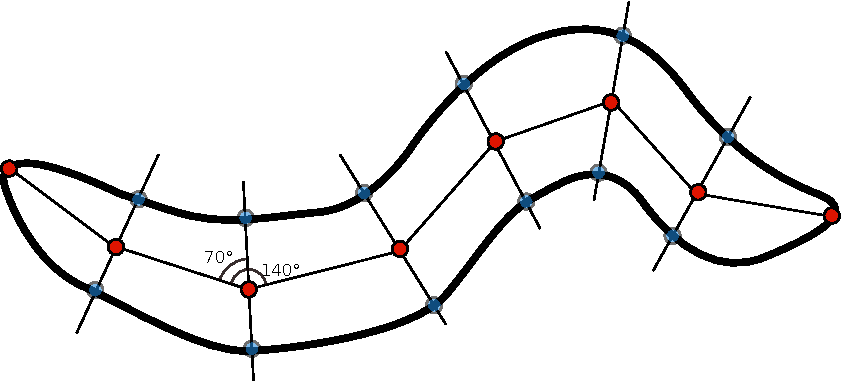
\includegraphics[scale=1]{descriptor/descriptor-vector.pdf}
 \caption{Construction of a worm shape based on shape descriptor}
 \label{fig:descriptor}
\end{figure}

Para obtener un contorno que represente una forma de gusano de manera precisa,
la escogencia de los puntos opuestos en las circunferencias de grosor
debe tomar en cuenta las flexiones del esqueleto. Dado que el contorno se
construye de acuerdo al grosor de los puntos control, las flexiones del gusano
a representar ocurren en cada uno de los puntos control. El grado de flexi\'on
de cada punto control se calcula como el \'angulo que existe entre las rectas
que conectan dicho punto con el punto anterior y posterior, respectivamente.\\

Por cada punto control, se calcula la bisectriz del \'angulo de flexi\'on y luego
se marcan los dos puntos opuestos donde se intersecan la bisectriz y la circunferencia
de grosor. Al calcular una curva que pasa por todos estos puntos, se obtiene un
contorno suave que modela una forma de gusano.\\

Generar una curva suave alrededor de los puntos control mejora la precisi\'on
de la forma descrita, en comparaci\'on con trazar l\'ineas rectas que
conecten los puntos de contorno. Esta representaci\'on permite modelar el 
contorno con m\'as detalle, utilizando un cantidad considerablemente menor
de puntos. La curva suave es obtenida calculando un \emph{spline} cardinal
(ver Sec. \ref{sec:splines}) dados los puntos contorno.\\

El perfil de gusanos para un conjunto de puntos control de tama\~no determinado 
puede ser, tanto definido manualmente, como calculado autom\'aticamente a partir
de los gusanos aislados, como se explica en el siguiente punto.


\subsubsection{Generaci\'on Autom\'atica de Perfiles}
\label{sec:metwormprof}

La forma de los gusanos aislados puede ser ajustada con precisi\'on, siguiendo
los puntos de contorno en el mapa de distancia, como se explica en la Sec. \ref{sec:metiso}.
Dado un conjunto de formas ajustadas de gusanos aislados y sus esqueletos respectivos, se 
puede generar un perfil de gusanos, midiendo el grosor de los puntos control y calculando
la media aritmetica de cada uno.\\

Para medir el grosor de cada punto control, se selecciona inicialmente un conjunto
de $N$ puntos equidistantes que cubren el esqueleto de un gusano aislado determinado.
Seguidamente, como se describe en la secci\'on previa, se calculan las bisectrices de los angulos
que existen entre las rectas que conectan los puntos control. A partir de cada punto control, 
se recorren los p\'ixeles de la bisectriz hasta que un punto de contorno es encontrado. Este
recorrido se hace en los dos sentidos, por lo que el proceso devuelve dos puntos de contorno.
A continuaci\'on, se calcula la distancia euclideana que existe desde cada punto control hasta
sus dos puntos opuestos respectivos, y se almacena el promedio de distancia.\\

Al repetir este proceso para cada gusano aislado se generan un conjunto de perfiles de gusanos
aislados, uno por cada gusano. A partir de este conjunto de perfiles, se calcula un perfil
general encontrando la media aritm\'etica de los valores de grosor por cada punto control.\\
Para que el perfil sea lo mas representativo posible, se descartan el $20\%$ de los gusanos
mas grandes y mas peque\~nos. El valor de grosor para los puntos extremos, \emph{i.e.} el
primer y \'ultimo punto en el conjunto de tama\~no $N$, es cero, por lo que en los extremos
solo se genera un punto de contorno, en vez de dos como en el resto de los puntos control.\\

Este proceso permite calcular entonces un perfil de grosor que define la distancia 
promedio de cada punto control a su punto de contorno mas cercano, haciendo posible
la generaci\'on de siluetas gen\'ericas de gusano alrededor de cualquier esqueleto.

\subsection{\emph{Rasterizaci\'on} de Siluetas}
\label{sec:metrast}

El enfoque de ajuste de formas se centra en minimizar la distancia entre siluetas
generadas y las formas de gusanos en la imagen. Para medir esta distancia se debe 
conocer el \'area de la silueta que es deformada.\\
El \'area de la silueta puede ser calculada a partir de su contorno. En t\'erminos
del tipo de datos que aqu\'i se manejan, el \'area consiste en el conjunto de p\'ixeles
que son cubiertos por la silueta, incluyendo los p\'ixeles de contorno.\\

El enfoque seguido para calcular el \'area consiste en dividir
en tri\'angulos el espacio definido por el contorno cerrado de la silueta y luego
\emph{rasterizar} cada tri\'angulo por separado. El t\'ermino \emph{rasterizar} se
refiere al proceso de transformar una im\'agen descrita en t\'erminos vectoriales
en un conjunto de p\'ixeles, de manera que pueda ser visualizada.\\

La descomposici\'on de un pol\'igono en tri\'angulos simples, es un problema
cl\'asico de computaci\'on gr\'afica. Diversas soluciones se han propuesto
como lo son: triangulaci\'on de Delaunay, triangulaci\'on de costo m\'inimo y
m\'etodo de \emph{ear clipping}, entre otros.
 
\subsubsection{Implementaci\'on}

El m\'etodo de \emph{ear clipping} fue escogido por su capacidad para triangular pol\'igonos
concavos y su sencillez de implementaci\'on. Para convertir el contorno del gusano en un 
pol\'igono, se transforma el \emph{spline} que lo define en un conjunto d\'iscreto de puntos.
Cada punto sucesivo es conectado a trav\'es de rectas, definiendo un pol\'igono cerrado. 
Para que la representaci\'on poligonal no afecte la suavidad del contorno definido por el
\emph{spline}, se escogen los puntos discretos (p\'ixeles) lo mas cerca posible uno de otros.
Seguidamente el contorno poligonal es triangulado.\\

Cada tri\'angulo es \emph{rasterizado} siguiendo el algoritmo de rasterizaci\'on por barrido
explicado en \cite{scanconversion}. El algoritmo consiste en \emph{rasterizar} 
l\'ineas horizontales entre los lados del triangulo hasta que el \'area es cubierta por completo.\\

Una vez \emph{rasterizados}, se pueden almacenar el \'area y el contorno de la silueta en
forma de datos manejables y visualizable. 

\subsection{Detecci\'on y Ajuste de Formas}
\label{sec:metfit}

Una vez que la imagen ha sido segmentada en diferentes grupos de gusanos, que se tiene
el esqueleto que representa el eje central de dichos grupos; y que se ha calculado un
perfil general de los gusanos en la imagen, se puede llevar a cabo el proceso de ajuste
de formas. Este proceso permite detectar los gusanos individuales que componen los 
diferentes grupos y almacenar sus formas respectivas en forma datos manejables y visualizables.\\

El proceso de detecci\'on y ajuste es diferente para cada tipo de grupos de gusanos: 
gusanos aislados y agrupaciones de gusanos. En esta secci\'on se explican las 
caracter\'isticas de este proceso en cada caso.

\subsubsection{Ajuste de Forma en Gusanos Aislados}
\label{sec:metiso}

En esta etapa de la metodolog\'ia, se conocen los diferentes gusanos aislados
y se tiene, por cada uno, un esqueleto delgado que conecta dos puntos
extremos de gusano a trav\'es de un camino.
Dado a que este proceso es llevado acabo despu\'es de que cada punto extremo
ha sido identificado correctamente y se conoce que el esqueleto no tiene
bifurcaciones, el \'area conformada por los p\'ixeles objeto del grupo
segmentado corresponder\'an a la forma exacta del gusano aislado en la
imagen.\\

Con el prop\'osito de tener una informaci\'on mas amplia acerca de los gusanos
detectados, se calcula tambi\'en el contorno a partir del \'area previamente identificada.
El contorno es trazado encontrando el p\'ixel de borde mas cercano a alg\'un punto extremo
del gusano y recorriendo cada p\'ixel de contorno vecino hasta cerrar el camino. 
Un p\'ixel de contorno es aquel que tiene el valor de uno (1) en el mapa de distancias.\\

Este proceso permite, entonces, obtener el contorno y el \'area de cada
gusano aislado en la imagen, de manera precisa.

\subsubsection{Worm Cluster shape fitting}
\label{sec:clusterfit}

The \emph{worm clusters} represent a more complicated shape matching scenario due to their
variable number of worms and the many different possible conformations that can be detected
on them. 
The  overlaps in \emph{worm clusters} makes difficult to differentiate the group of pixels
that belong to the area of one worm or another. A matching process must then be 
carried out that calculates the most likely worm conformation starting from every
endpoint in order to obtain the set of conformations that best fit the whole 
\emph{worm cluster}.\\

A shape optimization matching approach was followed that consists of calculating all the 
worm conformations starting from any endpoint. A worm conformation is obtained by generating
a generic worm shape from a skeleton path and deforming that shape until the dissimilarity
between the generated shape and the binary image is minimized. Below, the main steps and 
features of the algorithm are described:

\begin{itemize}
\item For every endpoint the set of feasible skeleton paths starting from that pixel
  are calculated.
\item Given a skeleton path, a generic worm shape is constructed by generating a shape
descriptor following the worm profile of the image.
\item An optimization process deforms the generic worm shape until the dissimilarity
between the shape and the corresponding binary image is minimized. The optimized
shape corresponds to a feasible worm conformation.
\item Once all the possible conformations from every endpoint are calculated, a set of
conformations is selected that maximizes the number of endpoints covered and minimizes
the sum of the energy values. The selected conformations are the best automatic matches.
\end{itemize}

\subsubsection*{Shape deformation}

The calculated skeleton paths, starting from a given endpoint, are guesses of possible
worm skeletons. Since the deformed model is constructed over a skeleton path 
(that is close to the medial axis of the \emph{worm cluster}) the initially generated 
shape will always be close to a worm shape. Given this, just slight perturbations of
the generated shape would deform the model sufficiently to correct the deviation of the
skeleton from the actual medial axis, obtaining thus the most likely worm shape
over the given path.\\

The deformations are made over a shape descriptor, which is defined by a series of 
control points and is constructed following a worm profile. In order to provide feasible
shapes and to limit the number of possible deformations, a deformation will consist
in the repositioning of a given control point. The number of different positions that a 
given control point can take is fixed and set along the bisection of the angle between
the lines that connect the previous, current and next control point. 
Following this, the set of deformations that can be performed from an initial shape 
can be calculated quickly and provides a great number of possible different conformations.\\

\subsubsection*{Energy Formulation}
 
The distance function must provide a measure of how far the deforming shape is from a worm in the image, 
\emph{i.e.} how well
the deforming shape fits. To measure the dissimilarity between a given worm shape and the
matching image, an energy formulation was followed, based on Active Contour Models,
\cite{snakes}, that consists of an external energy and an internal energy.\\

The external energy models how well the deformed model matches the data. Since the more
background pixels are covered the farther the model is from a worm in the \emph{worm cluster}, a good measure for the external energy would be the proportion of background pixels in the 
area covered by the deformed model. Then, the more object pixels are covered the lower the 
external energy is. So, given a model $M$ and the functions $bg$ and $fg$  that measure
the amount of background and foreground pixels respectively, the external energy
can be defined as:

$$E_{ext}(M) = \frac{bg(M)}{bg(M)+fg(M)}$$

The measure is not considered just as the sum of background pixels
because the energy value will be vary too much, given the variability of the amount
of pixels covered by a worm shape.\\

The internal energy is the one that models the objects resistance to be deformed into
a shape that do not corresponds to the modeling class, \emph{e.g.} the worm class. 
This means that the internal energy resists to obtain not feasible worm
shapes after deformation. The internal energy for
snakes, as explained in \cite{snakes}, works as a smoothness constraint and is explicitly
formulated (usually in terms of first and second derivatives). As stated in \cite{bspline}, 
many problems arising from this formulation have been recognized in literature such as:
slow convergence speed, difficulty in determining the weights associated with the 
smoothness constraint and possible inaccuracy in noisy environment of high order derivatives on discrete curves.\\
However, in the approach proposed in this work, every shape is generated from a worm 
profile following a shape descriptor, so every deformed shape will still belong to the 
worm class. Thus it is not necessary to include the internal energy in the 
formulation.

\subsubsection*{Matching Optimization}

The optimization process consists in obtaining the most likely worm shape that can be
obtained by deforming a shape constructed over a skeleton path, known as a 
worm conformation. Given how quickly a wide range of deformations can 
be computed, local-search is chosen as a metaheuristic for the optimization.
The process consists in obtaining the
best individual in the neighborhood that improves the energy function, until is 
minimized.
The neighborhood is calculated in the following way:
for a given shape, four (4) different deformations are calculated for control point.
The possible deformations or new positions are the
next and second next position in north and south direction, \emph{i.e. }the two opposites
directions of the bisection of the control point.
There are $N*4$ different possible deformations (neighbors) for a given shape,
where $N$ is the number of control points.\\ 
Then a neighborhood consists of mild and slightly stronger deformations of a given
worm shape for any control point.\\ Since the focus is to obtain the most accurate worm 
shape for a given skeleton, the
first and last control points, which correspond to the worm endpoints, are fixed.\\

Once the best shape is obtained, a contour fixing process is carried out. This
process consists in the expansion or contraction of areas of the shape contour, 
in order to adapt to the actual worm in the image. 
This is required since the optimized shape is built 
following a worm profile, which just represents the shape of 
the worms in the image generically. In this process, the extremes constructed from the control points are pushed
to contour points following the distance map, either expanding or contracting. While
expanding or contracting, every considered new possible position must have either the 
same or lower distance map value. A better point must be found after a fixed number
of steps, otherwise is discarded. This is done to avoid too big and strange deformations.

\subsubsection*{Conformations Assignment}

After the optimization process is performed, a subset of all the possible calculated 
conformations for \emph{worm clusters} must be selected, thus obtaining the image
worms match. The selected subset must maximize the number of endpoints covered and 
minimize the sum of energies of the conformations.\\
Any given endpoint may belong to at most one conformation. So, to any endpoint,
 there corresponds one and only one other endpoint. Therefore, the optimal subset of
conformations would be the minimal assignment between the sets of endpoints.\\
This can be obtained by solving the non-bipartite graph assignation problem. However,
given the implementation complexity (and possible performance overhead) of this algorithm,
a different algorithm  was designed. The implemented algorithm consists in a iterative 
greedy solution. The algorithm is applied for the sub clusters of \emph{worm clusters}. 
These sub clusters comprehend just the endpoints that are connected 
by feasible paths. The endpoints belonging to a given subcluster will be called 
conflicting endpoints.\\

The algorithm consists in the following:
Given $N$ conflicting endpoints a $NxN$ table is constructed indicating the cost
of the best conformation that connects an endpoint with another. Then, for a given starting row endpoint, the lowest value is selected and an assignment is made
between the row endpoint and the column endpoint (row and column are always different).
All the conformations starting from the row and column point are deleted.
Then, among the remaining rows, the one with the lowest value among the possible matches
is selected. The process is repeated after all the possible endpoints are assigned, thus
finding a solution. Once a solution is found, it is stored, the table is reconstructed and
the process is repeated starting from a different row, until all the rows have been taken
as starters. From all the gathered solutions, the one with the higher number of endpoints
covered and minimum total energy value is selected as the subcluster assignment.

\subsection{Manual Adjustment}
\label{sec:manualproc}

A process of manual adjustment can be performed by the user to improve the shape fitting
accuracy, such as adding missing endpoints or fixing wrong conformations. 
Below, both manual processes are explained. 

\subsubsection{Endpoint operations}
\label{sec:endpointop}

Worm endpoints are detected by first identifying extremes in the worm
skeleton. However, when the extreme of a given worm in the image overlaps with 
another worm shape, the shapes become continuous, so the shape skeleton will be generated 
as a continuous path. Thus, the extreme point will be missing and the endpoint will not be 
detected. Since the solution methodology is centered on finding paths between endpoints and 
then determining the most likely worm paths, having missing endpoints could affect 
the matching accuracy.\\

Worm endpoints are simple to detect for a human being, once had the skeleton of the 
a worm cluster, therefore the missing endpoints could be added quickly by following a manual
process. This process consists in looking at the extreme of worms and adding an 
extreme point when missing. Since by definition an endpoint is the extreme of a worm path,
it must have one and only one neighbor belonging to the skeleton. When an added extreme
point has more than one skeleton neighbor, the user would have to select the extra
neighbor pixel for deletion.
In summary the user can add the missing endpoints by selecting the missing pixel
and perhaps selecting some neighbors as well if it is necessary to disconnect. 

\subsubsection{Match Fixing}
\label{sec:matchfix}

After the optimization process is completed for the whole image, a set of 
worm conformations is given that corresponds to the best match assignation.
For some images there are worms that are not matched correctly, so 
conformations are given between incorrect pair of endpoints. 
Since in the optimization process all the possible conformations are calculated
between pair of endpoints, the wrong assignation could be fixed manually. A user
can recognize easily which conformations are incorrect, as well as quickly 
identify the endpoint that corresponds to any other endpoint. Then, by selecting 
the correct pair of endpoints, the corresponding
conformation will be modified, thus obtaining a correct fitting.
